\chapter{Software Architecture Design}
\label{chap:software-architecture-design}

\section{System Architecture Overview}
\label{section:architecture-overview}
The Prometheus system follows a distributed Edge-to-Cloud architecture designed to balance real-time performance with data scalability. The architecture is composed of four primary layers: the Data Ingestion Layer (IP Cameras), the Edge Processing Layer (Inference Engine), the Cloud Service Layer (Data Management), and the Presentation Layer (Client Applications).

As illustrated in Figure 4.1, the process begins at the edge to ensure low latency and privacy. Metadata is then pushed to the cloud to serve the analytical needs of gym owners and the real-time needs of members.

\begin{figure}[!ht]
    \centering
    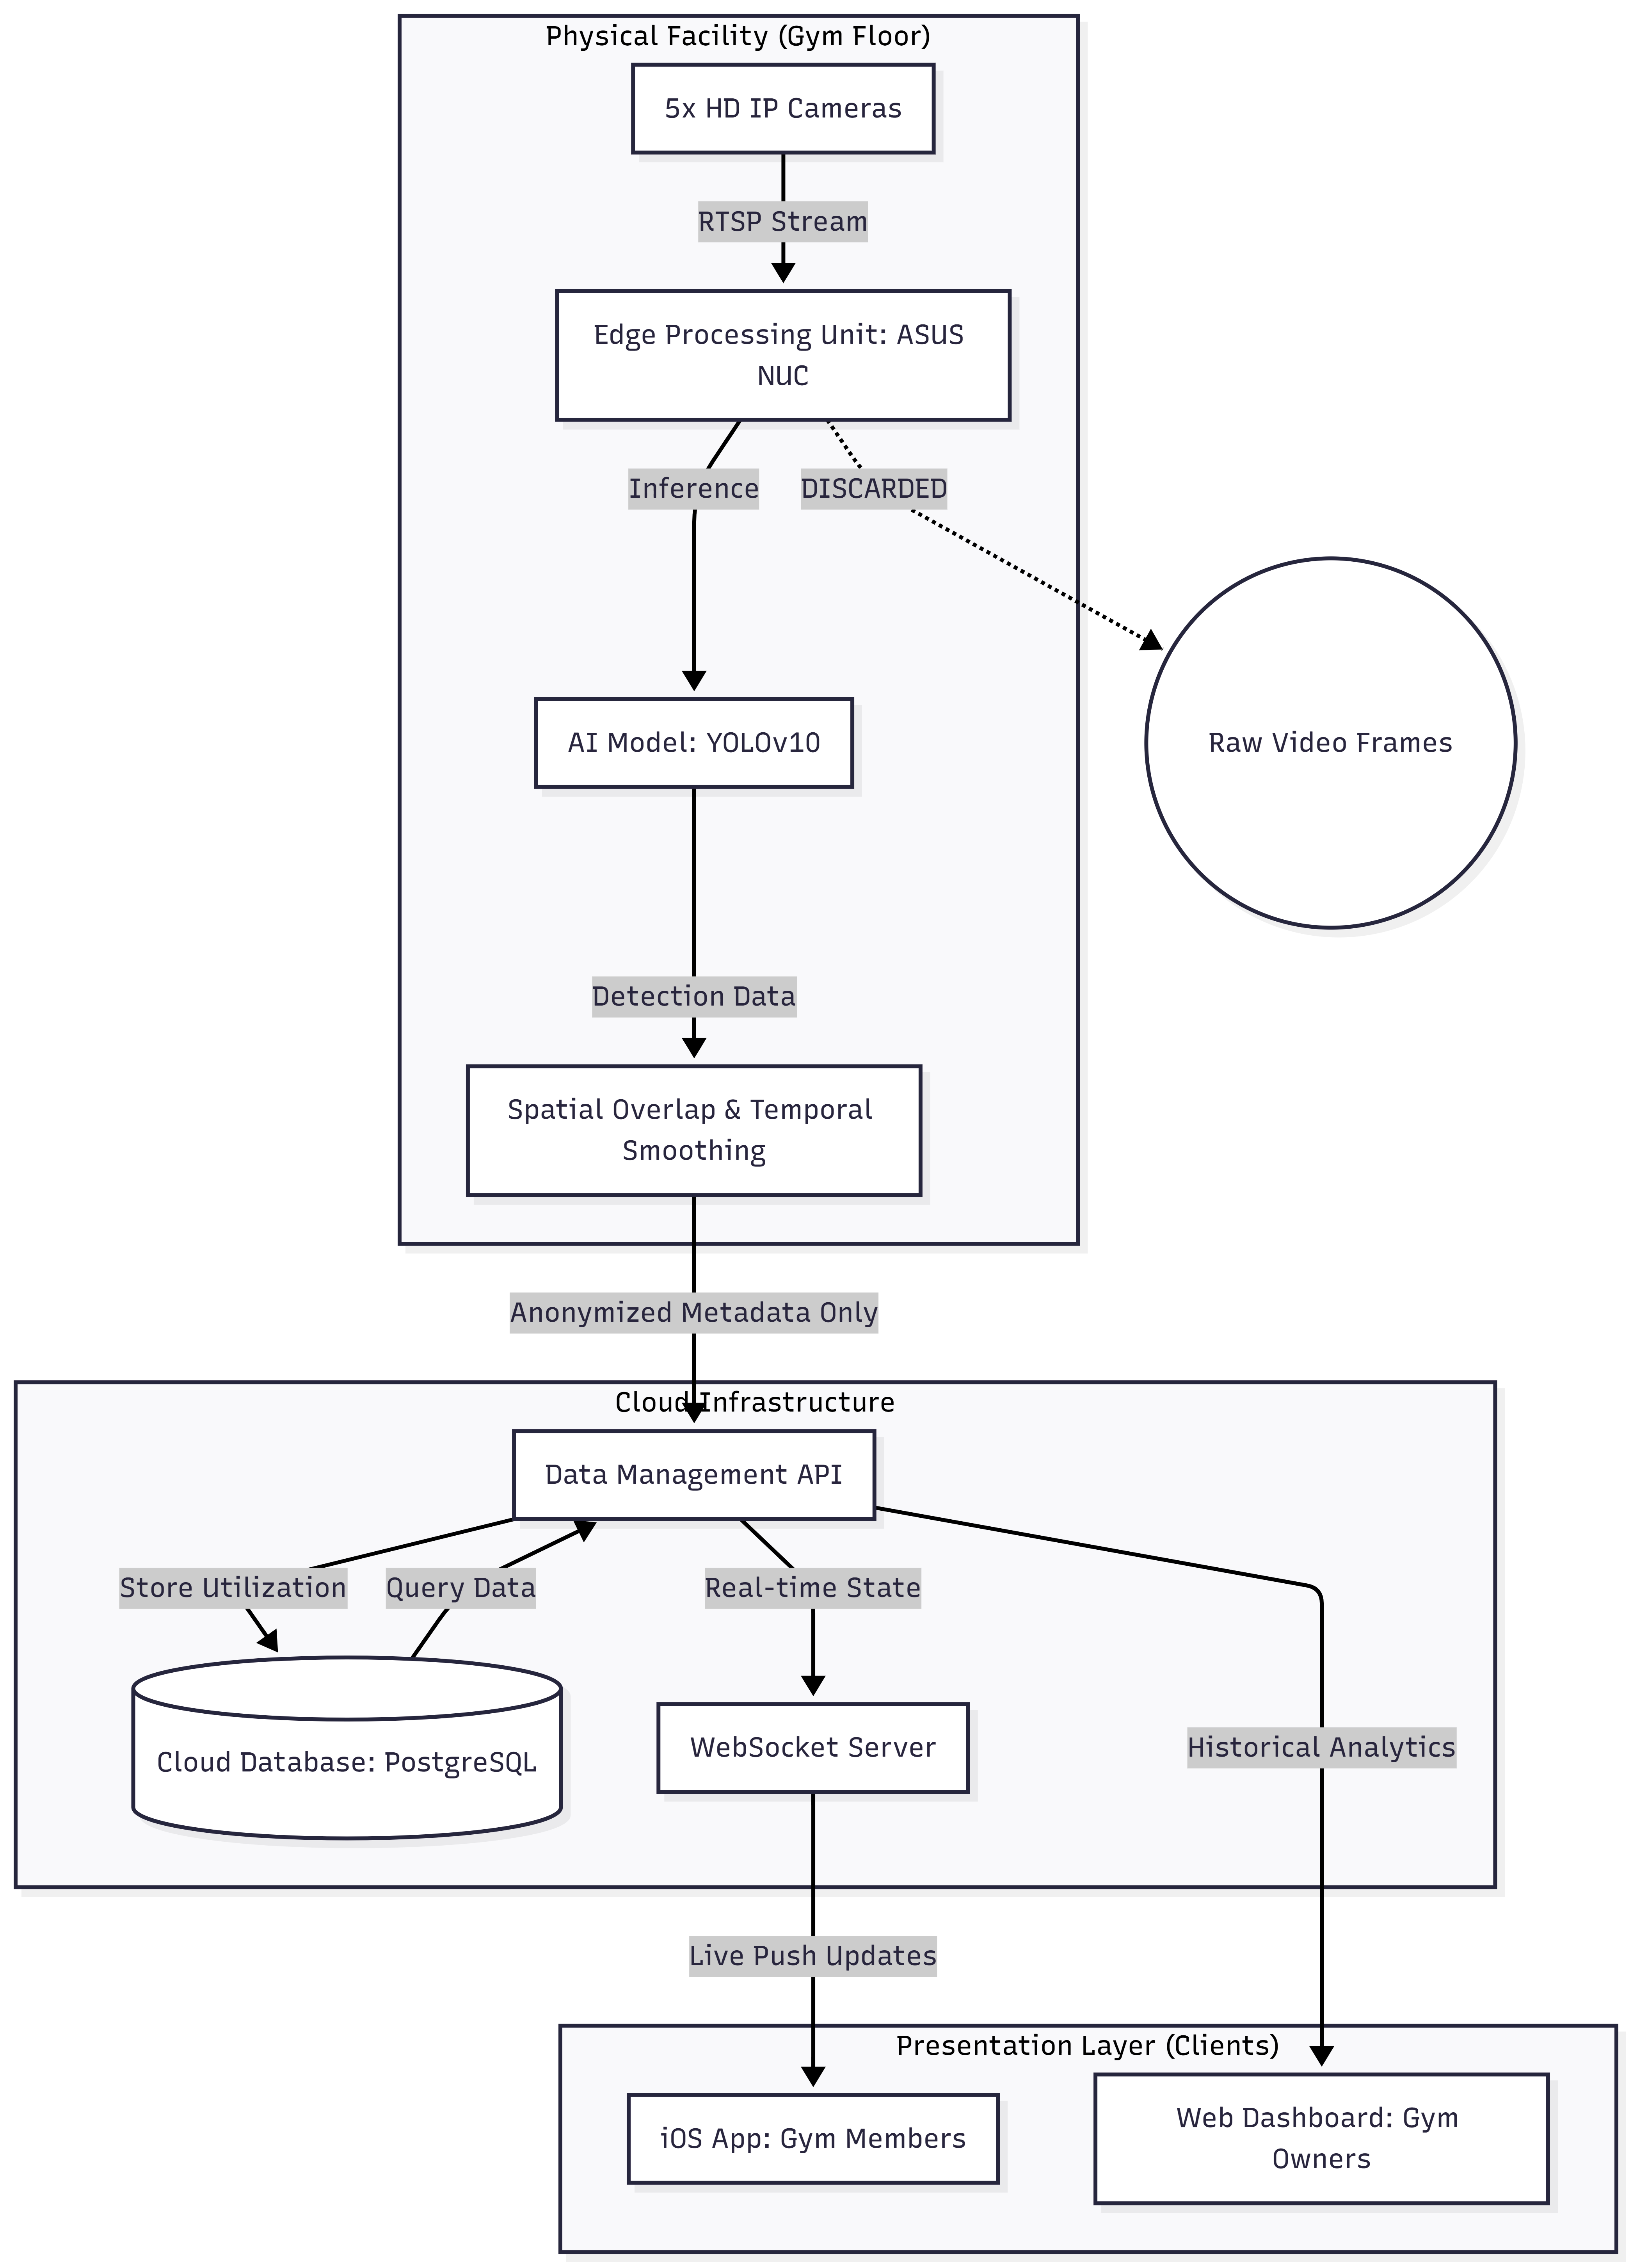
\includegraphics[width=\textwidth]{assets/figures/system-architecture.png}
    \caption{Prometheus Distributed Edge-to-Cloud System Architecture}
    \label{fig:system-architecture}
\end{figure}
\clearpage

The system begins with 5 HD IP cameras streaming high-definition video via RTSP to a local Edge Processing Unit (e.g., ASUS NUC). This unit performs real-time object detection and state classification, immediately discarding raw video frames to ensure member privacy. The resulting anonymized metadata is transmitted to a PostgreSQL-backed cloud database, which serves as the central repository for historical utilization data. Finally, the Presentation Layer delivers live availability updates to the iOS application and spatial heatmaps to the PC Web Dashboard.

\section{Software Design}
\label{section:software-design}
The runtime behavior of Prometheus is driven by a continuous inference loop. When a member interacts with a machine, the system must detect, validate, and broadcast this state change within seconds.

\textbf{Primary Sequence: Occupancy Update}
\begin{enumerate}
    \item The Edge Engine retrieves a frame and identifies "Person" and "Machine" objects using the YOLO model.
    \item The system applies a \textbf{Spatial Overlap Algorithm} to determine if a person is actively using a machine. This logic calculates the intersection of the person's bounding box with a pre-defined Region of Interest (ROI) for that specific machine.
    \item To prevent "flickering" from momentary occlusions or passersby, the system implements a \textbf{Temporal Smoothing} buffer: a state is only changed to "Occupied" if the overlap persists for at least 5 consecutive seconds.
    \item Once validated, the status is pushed to the cloud, triggering a WebSocket event that updates the machine's color on all active iOS client maps.
\end{enumerate}

\section{AI and Data Design}
\label{section:ai-data-design}

\subsection{Data Sources and Collection}
The Prometheus AI models are developed using a hybrid data strategy to ensure both general robustness and facility-specific accuracy:
\begin{itemize}
    \item \textbf{Public Benchmarks:} We utilize the M3GYM and QEVD datasets for baseline training. These sources provide millions of frames of traditional weightlifting and machine-based exercises from multiple CCTV-style angles.
    \item \textbf{Self-Collected Data:} To fine-tune the model for the specific layout of local facilities (such as the KEFF gym), we collect approximately 2,000 frames of facility-specific equipment.
    \item \textbf{Data Cleaning:} All training data undergoes perspective correction and manual annotation of "Free" vs. "Occupied" states. For privacy compliance, all human faces in the training set are blurred before being fed into the training pipeline.
\end{itemize}

\subsection{Model Design}
The core of the Prometheus intelligence is based on the \textbf{YOLO (You Only Look Once)} architecture. We have selected \textbf{YOLOv10} as the primary model for deployment on the ASUS NUC edge hardware. 
\begin{itemize}
    \item \textbf{Reasoning:} YOLOv10 was chosen over traditional R-CNN models because it offers the highest inference speed (frames per second) while maintaining the precision necessary for occupancy detection. Furthermore, YOLOv10's architecture eliminates Non-Maximum Suppression (NMS) overhead, which is critical for running multiple camera streams on a single edge device.
    \item \textbf{Integration:} The model is integrated into the system via an ONNX or TensorRT execution provider to maximize the utilization of the edge unit's GPU/NPU.
\end{itemize}

\subsection{Evaluation}
To ensure the system meets the established success criteria, the AI components are evaluated against the following metrics:
\begin{itemize}
    \item \textbf{Mean Average Precision (mAP):} To measure the model's accuracy in identifying machines and people.
    \item \textbf{State Accuracy:} The percentage of correctly identified "Free" vs. "Occupied" states, with a target of $\geq 95\%$.
    \item \textbf{End-to-End Latency:} The time elapsed from a person sitting on a machine to the iOS app reflecting the "Occupied" status. Target: $< 5$ seconds.
    \item \textbf{False Positive Rate:} The frequency at which the system incorrectly marks a machine as occupied due to environmental noise or passersby.
\end{itemize}